\documentclass[a4paper,12pt]{article}

\usepackage[utf8]{inputenc}

\usepackage[top=2.0cm,left=1.5cm,right=1.5cm,bottom=2.25cm]{geometry}
\linespread{1.5}

\usepackage{enumerate}

\usepackage[pdftex]{graphicx}

\usepackage{pifont}
\usepackage{listings}
\usepackage{xcolor}
\usepackage{listings}


\lstdefinestyle{BashStyle}{
  basicstyle=\small\sffamily,
  numbers=left,
  numberstyle=\footnotesize,
  numbersep=3pt,
  frame=tb,
  columns=fullflexible,
  backgroundcolor=\color{yellow!20},
  linewidth=0.9\linewidth,
  xleftmargin=0.1\linewidth
}

\lstdefinestyle{FileStyle}{
  basicstyle=\small\sffamily,
  numbers=left,
  numberstyle=\footnotesize,
  numbersep=3pt,
  frame=tb,
  columns=fullflexible,
  backgroundcolor=\color{blue!20},
  linewidth=0.9\linewidth,
  xleftmargin=0.1\linewidth
}

\usepackage{hyperref}

\usepackage{xcolor}
\definecolor{dark-red}{rgb}{0.4,0.15,0.15}
\definecolor{dark-blue}{rgb}{0.15,0.15,0.4}
\definecolor{medium-blue}{rgb}{0,0,0.5}

\hypersetup{
  colorlinks,
  linkcolor={dark-red},
  citecolor={dark-blue},
  urlcolor={medium-blue}
}

\reversemarginpar
\newcommand{\snote}[1]{\marginpar{\scriptsize{\begin{flushleft}#1\end{flushleft}}}}

\newcommand{\qpy}{\textsc{qpy}}

\usepackage{tikz}
\usetikzlibrary{positioning}

\begin{document}

\begin{titlepage}

\begin{center}
  qpy Manual
\end{center}\vspace{3.0cm}

% Titulo
\begin{center}
\begin{minipage}{0.9\textwidth}
\begin{center}
  {\textsf{\Large qpy - the \textbf{P}radipta's and \textbf{Y}uri's \textbf{PY}thon \textbf{Q}ueue system}}\\[0.5cm]
\end{center}
\end{minipage}
\end{center}

\begin{center}
{\large User, Administrator and Developer manual}
\end{center}

version X.X\\[3.0cm]

% Autor
\begin{flushleft}
Conceived and created by Pradipta Kumar Samanta and Yuri Alexandre Aoto\\\vspace{1.0cm}

With the kind help and support of Andreas K{\"o}hn and Arne Bargholz\\

\end{flushleft}



\vfill
% Fim da pagina
\begin{center}
{\large \today}
\end{center}

\end{titlepage}

%%% Local Variables:
%%% ispell-local-dictionary: "brasileiro"
%%% End:

\tableofcontents

\newpage
\section{For users}


\qpy{} is used to submit jobs from a main server and execute them in different nodes, according the availability or the choices given by the user.
It can handle jobs running in both single and multi processors and it has several options to make a friendly user interaction.
If you are using \qpy{} for the first time, please read carefully the section \ref{sec:basics}, \emph{Basics}, just bellow.
For a complete list of commands and their options, see the section \ref{sec:commands}, \emph{Commands}.


\subsection{Basics}\label{sec:basics}

\subsubsection{Installation}

The main instalation will probably be done by your system administrator.
You might have to do, however, the following thing:

Put the following lines in your $\sim$\texttt{/.bash\_profile} or $\sim$\texttt{/.bashrc}:


\begin{lstlisting}[style=FileStyle]
export PATH=<qpy_dir>:$PATH
source <qpy_dir>/bash_completion.sh
\end{lstlisting}

Your system administrador should tell you what is the \texttt{<qpy\_dir>} directory.
(S)He will might also send you a few files to be placed in your \qpy{} directory, $\sim$\texttt{/.qpy/}.
It's in this directory that 

\subsubsection{Initialisation}

The first \qpy{} command one should run is:

\begin{lstlisting}[style=BashStyle]
$ qpy restart
\end{lstlisting}

This command will set the background environment for using \qpy{}.
It should also be executed when some new update is done (you will be informed) or if the master node crashes.


\subsubsection{Basic concepts and usage}

Every job submmited by \qpy{} has an ID and a status.
The ID, a fixed integer for a particular job, is unique and identifies your job in the pool of jobs.
The status are:

\begin{itemize}
\item queue   - the job is waiting for allocation
\item running - the was allocated and is running
\item done    - the job have run and is finished
\item killed  - the job had its execution killed by the user
\item undone  - the job have not been executed (it was killed while in the queue)
\end{itemize}

When you just submit a job, it has the 'queue' status.
When a node is allocated for it, it is executed and the status changes to 'running'.
If the job terminates normally, the status changes to 'done'.
If you kills the job (that is, stops its execution), the status changes to 'killed'.
If you kills a job that is still on the queue, it will never be executed and the status changes to 'undone'.


You can submit a job using the sub command:

\begin{lstlisting}[style=BashStyle]
$ qpy sub <job's execution command>
\end{lstlisting}

This means that you put, on your queue of jobs, a new job that has to be executed with the command <job's execution command>.
\qpy{} will handle it for you from here on!

By the way, all commands in \qpy{} are like this:

\begin{lstlisting}[style=BashStyle]
$ qpy <cmd> [options]
\end{lstlisting}

where <cmd> is one of the \qpy{} commands and [options] are the otions for that command.
Of course, these options depend on the actual command <cmd>, some of them are optional, and so on.
See below for a complete list of commands and the explanation of their several options.

Now that your job is on the list, you probably want to be able to:
- check the status of your job (or jobs);
- check the situation of the nodes;
- eventually kill a unsatisfactory job.

This can be done by the following commands:

\begin{lstlisting}[style=BashStyle]
$ qpy check
\end{lstlisting}

This shows a list of all your jobs.
If you are interested only on a portion of these jobs, say, the ones that are currently running, try:

\begin{lstlisting}[style=BashStyle]
$ qpy check running
\end{lstlisting}

Another useful \qpy{} command is:

\begin{lstlisting}[style=BashStyle]
$ qpy status
\end{lstlisting}

It will show all the available node, users, how many jobs each one is running and so on.
If your jobs are for too long on the queue, this command should provide an indication why.

Sometimes we are not so happy with the development of a job and we want to terminate its execution, without waiting to its normal termination.
You can do this with:

\begin{lstlisting}[style=BashStyle]
$ qpy kill <job_ID>
\end{lstlisting}

where <job\_ID> is the ID number of the job.
Attention! This is not reversible.
\qpy{} will not ask you if you are sure to kill the job, so use the command with care.

There are several commands and options in \qpy{}.
Every command in \qpy{} can be completed automatically by using the TAB key.
It also gives the possible next arguments which, we hope, would be very helpful for all the users :)
For instance, if you type:

\begin{lstlisting}[style=BashStyle]
$ qpy kill ? <TAB> <TAB>
\end{lstlisting}

where \texttt{<TAB> <TAB>} indicates that you should type the \texttt{TAB} key two times, you will receive a brief explanation on the command sub.



\subsection{Commands}\label{sec:commands}


The followings are all the commands of \qpy{}.
The user can run any of these commands as

\begin{lstlisting}[style=BashStyle]
$ qpy <cmd> [options]
\end{lstlisting}

where \texttt{[options]} depends on the actual command \texttt{<cmd>}.


\subsubsection{restart}

The user can start \qpy{} background environment with this command.
This command also works as an easy way to finish current session of \qpy{} and start a new, which is most useful when the user wants to update the \qpy{} to its latest version.

\begin{itemize}
\item Options:
  there are no options.

\item Examples:

  Restart the \qpy background environment:

\begin{lstlisting}[style=BashStyle]
$ qpy restart
\end{lstlisting}

\end{itemize}  

\subsubsection{finish}

If you feel like done using \qpy{}, please finish the existing \qpy{} environment which is running in background using this command.
If somehow the qpy-master crashes while using, please remove the '.port' file from the \qpy{} directory before starting a new \qpy{} session. 

\begin{itemize}
\item Options:
  there are no options.
  
\item Examples:
  
  Finishes the background \qpy{} environment:

\begin{lstlisting}[style=BashStyle]
$ qpy finish
\end{lstlisting}
  
\end{itemize}


\subsubsection{sub}

Submit any executable after the command 'qpy sub'.
The output and the error file of running that particular script will be written in the files 'job\_<job\_ID>.out' and 'job\_<job\_ID>.err' respectively.

Submitting a serial job is the default one for this command.
To submit a job that uses multi-processor, please add the information of number of processors (N) needed either by putting '-n N' between 'qpy sub' and the executable, or by adding '\#QPY n\_cores=N' in the script running.
For the first case, do not put the option after the executable as it would then be considered as an option corresponding to the executable. 

\qpy{} also check if enough memory is available in a node before starting a job there.
The defualt memory it checks for availibility is 5 GB. If a job needs to use more memory (M) please add this information either by putting '-m M' between 'qpy sub' and the executable, or by adding '\#QPY mem=M' in the script running.


\begin{itemize}
\item Options:
  the executable and its arguments;
  optionally, the the following flags BEFORE the executable:

    -n <n cores>        the number of cores
    -m <memory>         requested memory, in GB


\item Examples:

  Executes the command 'hostname'. Allocates one cores and 5 GB of memory for it (default values):

\begin{lstlisting}[style=BashStyle]
$ qpy sub hostname
\end{lstlisting}
  
  Executes the script './script.sh'. Allocates three cores and 10 GB of memory for it:

\begin{lstlisting}[style=BashStyle]
$ qpy sub -n 3 -m 10 ./script.sh 
\end{lstlisting}
  Executes the command 'ls -ltr':

\begin{lstlisting}[style=BashStyle]
$ qpy sub ls -ltr
\end{lstlisting}

\end{itemize}
  
\subsubsection{check}

Check the status of all the submitted jobs.
The command 'qpy check' gives the list of all jobs submitted.
One can also check jobs of specific status which are: 'running', 'done', 'killed', 'undone' and 'queue' adding the keyword after 'qpy check'


\begin{itemize}

\item Options:
  a status
  a job ID list
  
\item Examples:

\end{itemize}

\subsubsection{kill}

Kill a particular jobs using the command 'qpy kill [jobid]'. One can also kill several jobs by providing a list of jobid's or a range of jobid's separated by '-'. Kill 'all'/'running' jobs or jobs in 'queue' by replacing the [jobid] with these keywords. 


\begin{itemize}
\item Options:
  a status ('queue' or 'running')

  a job ID list

  'all'  

\item Examples:

\end{itemize}


\subsubsection{status}

This command is mainly useful for the 'multi-user' environment.
It writes elaborately the number of jobs running for each users and in each of the available nodes. 

\begin{itemize}
\item Options:
  There are no options.
  
\item Examples:

\end{itemize}


\subsubsection{config}

This command gives informations about some of the variables in \qpy{}.
Feel free to check.
It is quite self explanatory.
One of the advanced feature of this command is to configure the format that 'qpy check' would follow.
The default format that 'qpy check' uses to write all the jobs is '%j (%s):%c (on %n; wd: %d)\n'.

It might seem little complicated, but it follows mainly these rules:

\begin{itemize}
\item \%j : job ID
\item \%s : job status
\item \%c : command you used to submit the job
\item \%d : working directory of your job
\item \%n : node allocated for your job
\item \%N : number of cores for your job.
\item \%R : running time of the job. (time in queue if the job is in queue)
\item \%Q : actual time when the job is submitted
\item \%S : actual time when the job has started
\item \%E : actual time when the job has finished
\end{itemize}

The user can also change this format to a minimalistic one, by 'qpy config checkFMT \%j:\%s' or anything using the notations defined above. To check the current format, use the command 'qpy config checkFMT' and to change it to the default one, use 'qpy config checkFMT default'.

There are some new options available to format 'qpy check' and have some information about the timing of the jobs. These are:


Bash scripts, generally, stops if changes are made in it while it is still running.
So it is better to have \qpy{} running a copied script which allows to change and reuse the original bash script.
'qpy config' provides another advanced option to do this by copying the script to the local folder '~/.qpy/scripts' and use it later while running the actual calculation.
This is very useful while working with a bash script.
To use this, set it up with 'qpy config copyScripts true', where by default 'copyScripts' is set to 'false'. 

The same thing can also be done for a specific job if the submitted scipt has the line '\#QPY cpScript true' or if the job is submitted using the command 'qpy sub -c [script\_name]'.
If the 'copyScripts' is set True, then the reverse can be done by adding the line '\#QPY cpScript false' in the script or by submitting the script using the command 'qpy sub -o [script\_name]'.


\begin{itemize}

\item Options: % Write some options...

  
\item Examples:

\end{itemize}

\subsubsection{ctrlQueue}

ctrlQueue is a command to control and move the jobs in the queue.
Consider the situation where you  have a long list of jobs in the queue but you have some job(s) of top priority that needs to be done as soon as possible.
The command ctrlQueue can be used in this situtation to move the priority job(s) up in the queue-list.
These are what you have to follow:

'qpy ctrlQueue pause' : This command needs to be used prior to moving the jobs. This command ensures that no jobs from the queue can be started further. 

'qpy ctrlQueue jump [job-id-1] [job-id-2] [job-id-3] ... [job-id-n] [job-id-pos]' : This is the main command for moving the jobs. Here all the jobs (1 to n) are moved in the queue to be placed after [job-id-pos] in the queue-list. 

'qpy ctlrQueue continue' : This command remove the pause and let \qpy{} to continue putting jobs from queue to the nodes. 

\begin{itemize}

\item Options:

\item Examples:

\end{itemize}

\subsubsection{clean}

It cleans the list of jobs that one can see using 'qpy check'.
The user can clean some specific jobs by adding the job id or the specific status of the job.
The jobs that can be cleaned are 'done', 'killed' and 'undone'. 


\begin{itemize}

\item Options:
  a status ('done', 'killed' or 'undone')
  a job ID list
  'all'  

\item Examples:

\end{itemize}

\subsubsection{tutorial}

Shows a tutorial.

\begin{itemize}
\item Options:

\item Examples:

\end{itemize}



\newpage
\section{For administrators}

The duties of the administrator of \qpy{} are basic to maintain the program ``qpy-multiuser'' running and add/remove new users and machines.
This section explains how this is done.

\subsection{Installation}\label{sec:instal_admin}

We assume that you have a copy of \qpy{}, otherwise you wouldn't be reading this manual.
To set up a new \qpy{} environment, create the following directory in the administrator's home directory:

\begin{lstlisting}[style=BashStyle]
$ mkdir ~/.qpy-multiuser/
\end{lstlisting}
And create the following files:

\begin{verbatim}
~/.qpy-multiuser/distribution_rules
~/.qpy-multiuser/allowed_users
~/.qpy-multiuser/nodes
~/.qpy-multiuser/multiuser_connection_address
\end{verbatim}

The content of these files are described in section \ref{sec:files_admin}.
Create them according to your local needs.
After this, start the qpy-multiuser with:

\begin{lstlisting}[style=BashStyle]
$ python ${QPY_DIR}/qpy-access-multiuser.py start
\end{lstlisting}


\subsection{Add new user}

To add a new user in \qpy{}, first add his name in the file

\begin{verbatim}
~/.qpy-multiuser/allowed_users
\end{verbatim}

After, you have to send the following files to the new user:

\begin{verbatim}
~/.qpy-multiuser/multiuser_connection_address
~/.qpy-multiuser/multiuser_connection_port
~/.qpy-multiuser/multiuser_connection_conn_key
\end{verbatim}

These should be placed in the user's \qpy{} directory:

\begin{verbatim}
${USER}/.qpy/multiuser_connection_address
${USER}/.qpy/multiuser_connection_port
${USER}/.qpy/multiuser_connection_conn_key
\end{verbatim}

In addition, if you have a dedicated machine to run \qpy{}, add this file to the user's \qpy{} directory:

\begin{verbatim}
${USER}/.qpy/master_connection_address
\end{verbatim}

with the address of the machine where his qpy-master is supposed to run.
If this file is not present, \qpy{} runs locally.

\subsection{Add and remove a node}

To add a new node, add a new line in the file

\begin{verbatim}
~/.qpy-multiuser/nodes
\end{verbatim}

with the information about the node (see section \ref{sec:files_admin} for a description of this file).
Then run:

\begin{verbatim}
$ python ${QPY_DIR}/qpy-access-multiuser.py nodes
$ python ${QPY_DIR}/qpy-access-multiuser.py distribute
\end{verbatim}




\subsection{Update version}

When a new version of \qpy{} is released, depending where the new changes have been done, you might have to restart the qpy-multiuser:

\begin{verbatim}
$ python ${QPY_DIR}/qpy-access-multiuser.py finish
$ python ${QPY_DIR}/qpy-access-multiuser.py start
\end{verbatim}

And/or ask all the users to restart their qpy-masters.
Whatever is the case, this will be informed in the release's notes.



\subsection{Commands}

This is a full list of the commands that are available to the administrator:

\begin{lstlisting}[style=BashStyle]
$ python ${QPY_DIR}/qpy-access-multiuser.py start
\end{lstlisting}

Starts a new qpy-multiuser instance.
Run this if you are starting \qpy{} for the first time, if a update is needed or if the machine qhere \qpy{} runs has crashed.

\begin{lstlisting}[style=BashStyle]
$ python ${QPY_DIR}/qpy-access-multiuser.py finish
\end{lstlisting}

Finishes the qpy-multiuser program

\begin{lstlisting}[style=BashStyle]
$ python ${QPY_DIR}/qpy-access-multiuser.py nodes
\end{lstlisting}

Loads the content of the \texttt{nodes} file.

\begin{lstlisting}[style=BashStyle]
$ python ${QPY_DIR}/qpy-access-multiuser.py distribute
\end{lstlisting}

Distribute the cores among the users.

\begin{lstlisting}[style=BashStyle]
$ python ${QPY_DIR}/qpy-access-multiuser.py variables
\end{lstlisting}

Lists several internal variables of qpy-multiuser.
Used mainly to check if something is going wrong.

\begin{lstlisting}[style=BashStyle]
$ python ${QPY_DIR}/qpy-access-multiuser.py status
\end{lstlisting}

Show the current status of the users, nodes and cores.

\begin{lstlisting}[style=BashStyle]
$ python ${QPY_DIR}/qpy-access-multiuser.py saveMessages
\end{lstlisting}

Saves messages from the internals of qpy-multiuser, that will be shown in the ``variables'' command.
Mainly for debugging purposes.

\textbf{ATTENTION!}

The next commands are not supposed to be used in a normal run.
Use them only if you know exactly what you are doing.

\begin{lstlisting}[style=BashStyle]
$ python ${QPY_DIR}/qpy-access-multiuser.py __user <user_name> <address> <port> <conn_key>
\end{lstlisting}

Adds a new user to qpy-multiuser.

\begin{lstlisting}[style=BashStyle]
$ python ${QPY_DIR}/qpy-access-multiuser.py __req_core <user_name> <jobID> <n_cores> <mem> <queue_size>
\end{lstlisting}

Requires a core from qpy-multiuser.

\begin{lstlisting}[style=BashStyle]
$ python ${QPY_DIR}/qpy-access-multiuser.py __remove_job <user_name> <job_ID> <queue_size>
\end{lstlisting}

Removes a job from qpy-multiuser.



\subsection{Files}\label{sec:files_admin}

This is a list of the files in the qpy-multiuser directory.

\begin{verbatim}
~/.qpy-multiuser/distribution_rules
\end{verbatim}

This file defines how the cores are distributed to the users.
The basic syntax is one of the following:

\begin{lstlisting}[style=FileStyle]
even minimum <n_cores>
\end{lstlisting}

This means an even distribution among the users, with at least \texttt{n\_cores} granted for each.

\begin{verbatim}
~/.qpy-multiuser/allowed_users
\end{verbatim}

A list with all the users that can use the current qpy environment:

\begin{lstlisting}[style=FileStyle]
<user_1>
<user_2>
<user_3>
\end{lstlisting}

\begin{verbatim}
~/.qpy-multiuser/nodes
\end{verbatim}

A list with all the nodes available in the qpy environment.
Each line has: hostname of the node, followed by the number of cores this node has (or is available to \qpy{}) and, optionally, a ``M'', to indicate that that node has preference for multicore jobs.

\begin{lstlisting}[style=FileStyle]
<node_1> <n_cores> [M]
<node_2> <n_cores> [M]
<node_3> <n_cores> [M]
\end{lstlisting}

\begin{verbatim}
~/.qpy-multiuser/multiuser_connection_address
\end{verbatim}

The address where the qpy-multiuser instance will run.
If you do not set this, \qpy{} automatically uses the local machine.

\begin{lstlisting}[style=FileStyle]
<machine_address>
\end{lstlisting}


The following files are generated and used by \qpy{}, but the administrator should not alter or delete them.
They have the information required to make all the message transfers.

\begin{verbatim}
~/.qpy-multiuser/multiuser_connection_port
~/.qpy-multiuser/multiuser_connection_key
~/.qpy-multiuser/connection_<user>_key
~/.qpy-multiuser/connection_<user>_key
~/.qpy-multiuser/connection_<user>_key
\end{verbatim}









\newpage
\section{For developers}


% Fixed behaviours: environment variables and other things that should never change.

% Typical ideas of the code: main classes and threads


%\textbf{\Large Fluxograma do projeto}\label{fluxograma}
\linespread{0.8}

\begin{center}
%\footnotesize
  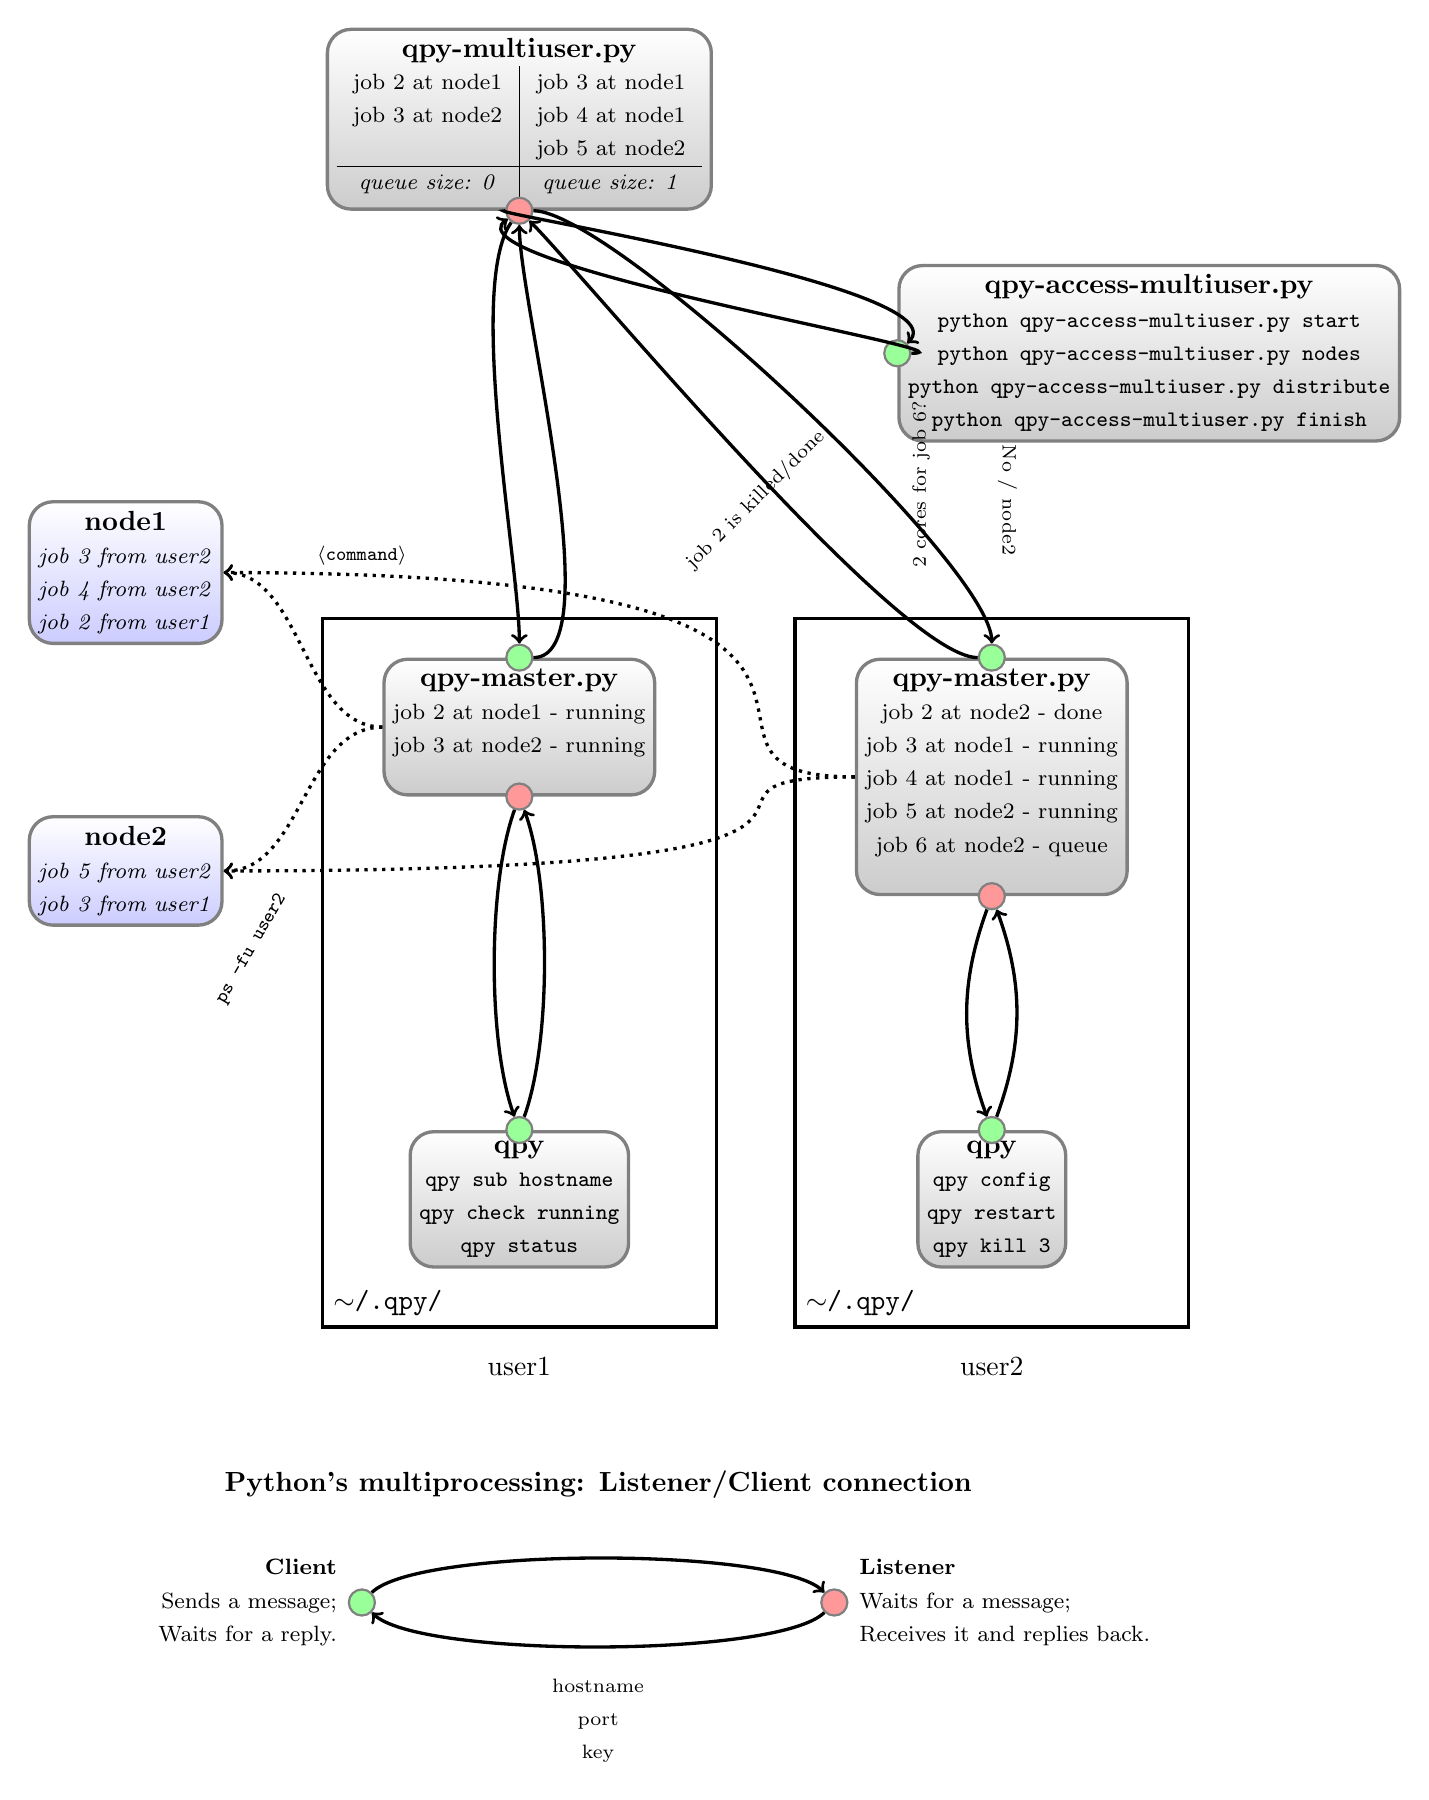
\begin{tikzpicture}[
    ->,
    double,
    very thick,
    program/.style={
      align=center, anchor=north,
      rectangle,minimum size=6mm,rounded corners=3mm,
      very thick,draw=black!50,
      top color=white,bottom color=black!20
    },
    comp/.style={
      align=center, anchor=north,
      rectangle,minimum size=6mm,rounded corners=3mm,
      very thick,draw=black!50,
      top color=white,bottom color=blue!20
    },
    list/.style={
      align=center, anchor=center,
      circle,minimum size = 0.3cm,
      thick,draw=black!50,
      fill=red!40
    },
    client/.style={
      align=center, anchor=center,
      circle,minimum size = 0.3cm,
      thick,draw=black!50,
      fill=green!40
    }
    ]

    \node (multiuser)  at (-3.0,3.0)[program] {
      \textbf{qpy-multiuser.py}\\
      \begin{tabular}{c|c}
        {\footnotesize job 2 at node1} & {\footnotesize job 3 at node1}\\
        {\footnotesize job 3 at node2} & {\footnotesize job 4 at node1}\\
        &{\footnotesize job 5 at node2}\\
        \hline
        \textit{\footnotesize queue size: 0}&\textit{\footnotesize queue size: 1}
      \end{tabular}
    };
    \node (multiuser_list) at (multiuser.south) [list] {};

    \node (access)  at (5.0,0.0)[program] {
      \textbf{qpy-access-multiuser.py}\\
      \texttt{\footnotesize python qpy-access-multiuser.py start}\\
      \texttt{\footnotesize python qpy-access-multiuser.py nodes}\\
      \texttt{\footnotesize python qpy-access-multiuser.py distribute}\\
      \texttt{\footnotesize python qpy-access-multiuser.py finish}
    };
    \node (access_client) at (access.west) [client] {};

    \draw [->] (multiuser_list.180) .. controls ++(180:0.4) and ++(45:1) .. (access_client.45);
    \draw [->] (access_client.0) .. controls ++(0:1) and ++(+215:1) .. (multiuser_list.215);

    \node (master1)  at (-3.0,-5.0)[program] {
      \textbf{qpy-master.py}\\
      {\footnotesize job 2 at node1 - running}\\
      {\footnotesize job 3 at node2 - running}\\
    };
    \node (master1_client) at (master1.north) [client] {};
    \node (master1_list) at (master1.south) [list] {};

    \draw [->] (master1_client.0) .. controls ++(0:1) and ++(-90:1) .. (multiuser_list.-90);
    \draw [->] (multiuser_list.+235) .. controls ++(+235:1) and ++(+90:1) .. (master1_client.90);
    
    \node (master2)  at (3.0,-5.0)[program] {
      \textbf{qpy-master.py}\\
      {\footnotesize job 2 at node2 - done}\\
      {\footnotesize job 3 at node1 - running}\\
      {\footnotesize job 4 at node1 - running}\\
      {\footnotesize job 5 at node2 - running}\\
      {\footnotesize job 6 at node2 - queue}\\
    };
    \node (master2_client) at (master2.north) [client] {};
    \node (master2_list) at (master2.south) [list] {};

    \draw [->] (master2_client.180) .. controls ++(180:1) and ++(-45:1) .. (multiuser_list.-45);
    \draw [->] (multiuser_list.0) .. controls ++(0:1) and ++(+90:1) .. (master2_client.90);


    \node (qpy1)  at (-3.0,-11.0)[program] {
      \textbf{qpy}\\
      \texttt{\footnotesize qpy sub hostname}\\
      \texttt{\footnotesize qpy check running}\\
      \texttt{\footnotesize qpy status}
    };
    \node (qpy1_client) at (qpy1.north) [client] {};

    \node (qpy2)  at (3.0,-11.0)[program] {
      \textbf{qpy}\\
      \texttt{\footnotesize qpy config}\\
      \texttt{\footnotesize qpy restart}\\
      \texttt{\footnotesize qpy kill 3}
    };
    \node (qpy2_client) at (qpy2.north) [client] {};

    \node (node1)  at (-8.0,-3.0)[comp] {
      \textbf{node1}\\
      \textit{\footnotesize job 3 from user2}\\
      \textit{\footnotesize job 4 from user2}\\
      \textit{\footnotesize job 2 from user1}
    };

    \node (node2)  at (-8.0,-7.0)[comp] {
      \textbf{node2}\\
      \textit{\footnotesize job 5 from user2}\\
      \textit{\footnotesize job 3 from user1}
    };

    
    \draw [->] (qpy1_client.70) .. controls ++(70:1) and ++(-70:1) .. (master1_list.-70);
    \draw [->] (master1_list.-110) .. controls ++(-110:1) and ++(+110:1) .. (qpy1_client.110);
    
    \draw [->] (qpy2_client.70) .. controls ++(70:1) and ++(-70:1) .. (master2_list.-70);
    \draw [->] (master2_list.-110) .. controls ++(-110:1) and ++(+110:1) .. (qpy2_client.110);
    
    
    \node [rotate=45] at (0.0,-3.0) {\scriptsize job 2 is killed/done};
    \node [rotate=90] at (2.1,-2.8) {\scriptsize 2 cores for job 6?};
    \node [rotate=-90] at (3.2,-3.0) {\scriptsize No / node2};
 
    \node at (-5,-3.7) {\texttt{\scriptsize $\langle$command$\rangle$}};
    \node [rotate=60] at (-6.4,-8.7) {\texttt{\scriptsize ps -fu user2}};

    \draw [->,dotted] (master1.-180) .. controls ++(-180:1) and ++(0:1) .. (node1.0);
    \draw [->,dotted] (master1.-180) .. controls ++(-180:1) and ++(0:1) .. (node2.0);
    \draw [->,dotted] (master2.-180) .. controls ++(-180:3) and ++(0:10) .. (node1.0);
    \draw [->,dotted] (master2.-180) .. controls ++(-180:3) and ++(0:10) .. (node2.0);
    
    
    \draw [] (-5.5, -4.5) rectangle (-0.5,-13.5);
    \draw [] (0.5, -4.5) rectangle (5.5,-13.5);
    \node [anchor=west] at (-5.5,-13.2) {$\sim$\texttt{/.qpy/}};    
    \node [anchor=west] at (0.5,-13.2) {$\sim$\texttt{/.qpy/}};    
    \node at (-3.0,-14.0) {user1};
    \node at (3.0,-14.0) {user2};
    
    
    
    \node at (-2.0,-15.5) {\textbf{Python's multiprocessing: Listener/Client connection}};
    \node [align=center] at (-2.0,-18.5) {\scriptsize hostname\\\scriptsize port\\\scriptsize key};
    
    \node (client_templ) [client] at (-5.0,-17.0){};
    \node (list_templ) [list] at (1.0,-17.0){};
    \node [anchor=east, align = right] at (client_templ.west) {
      \textbf{\footnotesize Client}\\
      {\footnotesize Sends a message;}\\
      {\footnotesize Waits for a reply.}
    };
    \node [anchor=west, align = left] at (list_templ.east) {
      \textbf{\footnotesize Listener}\\
      {\footnotesize Waits for a message;}\\
      {\footnotesize Receives it and replies back.}
    };
    
    \draw [->] (client_templ) .. controls ++(45:1) and ++(135:1) .. (list_templ);
    \draw [->] (list_templ) .. controls ++(-135:1) and ++(-45:1) ..  (client_templ);
    






% Grid
     % \foreach \y in {-15,...,2} {
     %   \node at (-9,\y) {\y};
     %   \draw [-] [dotted] (-8.5,\y) -- (5.0,\y);
     % };
     % \foreach \x in {-5,...,5} {
     %   \node at (\x,-18.5) {\x};
     %   \draw [-] [dotted] (\x,-18.0) -- (\x,2);
     % };
    

    
  \end{tikzpicture}
\end{center}

\linespread{1.5}



\end{document}

%%% Local Variables:
%%% ispell-local-dictionary: "british"
%%% mode: latex
%%% TeX-master: t
%%% End: 
